%  LaTeX support: latex@mdpi.com
%  For support, please attach all files needed for compiling as well as the log file, and specify your operating system, LaTeX version, and LaTeX editor.

%=================================================================
\documentclass[foods,article,submit,moreauthors]{Definitions/mdpi}
% The class option "submit" will be changed to "accept" by the Editorial Office when the paper is accepted.

%=================================================================
% MDPI internal commands - do not modify
\firstpage{1}
\makeatletter
\setcounter{page}{\@firstpage}
\makeatother
\pubvolume{1}
\issuenum{1}
\articlenumber{0}
\pubyear{2026}
\copyrightyear{2026}
%\externaleditor{Firstname Lastname}
\datereceived{ }
\daterevised{ } % Comment out if no revised date
\dateaccepted{ }
\datepublished{ }
%\datecorrected{}
%\dateretracted{}

%=================================================================
% Add packages and commands here. The following packages are loaded in our class file: fontenc, inputenc, calc, indentfirst, fancyhdr, graphicx, epstopdf, lastpage, ifthen, float, amsmath, amssymb, lineno, setspace, enumitem, mathpazo, booktabs, titlesec, etoolbox, tabto, xcolor, colortbl, soul, multirow, microtype, tikz, totcount, changepage, attrib, upgreek, array, tabularx, pbox, ragged2e, tocloft, marginnote, marginfix, enotez, amsthm, natbib, hyperref, cleveref, scrextend, url, geometry, newfloat, caption, draftwatermark, seqsplit
\usepackage{longtable}
\usepackage{bm}

% Placeholder for information that only the authors can supply.
% All \tbc{...} items must be completed and the macro removed before upload
% (check: grep -n tbc *.tex).
\newcommand{\tbc}[1]{\textcolor{red}{[TO BE COMPLETED: #1]}}

%=================================================================
% Full title of the paper (Capitalized)
\Title{Reproducibility of Honey Taste and Odor Typicality Assessment: A Blind Consumer Panel Versus the Verdicts of Four Laboratories}

% Author Orchid ID: enter ID or remove command
\newcommand{\orcidauthorA}{0009-0004-1158-0693} % Bartosz Lewandowski
\newcommand{\orcidauthorB}{0009-0003-7214-4097} % Przemysław Rujna
\newcommand{\orcidauthorC}{0000-0001-9178-1540} % Katarzyna Joanna Banach
\newcommand{\orcidauthorD}{0000-0003-2580-7954} % Ewaryst Tkacz
\newcommand{\orcidauthorE}{0000-0003-3900-7368} % Anna Gajda
\newcommand{\orcidauthorF}{0000-0003-1865-2122} % Maciej Wróbel
\newcommand{\orcidauthorG}{0000-0002-6289-7234} % Radosław Dzik
\newcommand{\orcidauthorH}{0000-0002-3575-8159} % Agata Kabała-Dzik
\newcommand{\orcidauthorI}{0009-0006-2931-1867} % Julia Rujna

% Authors, for the paper (add full first names)
\Author{Bartosz Lewandowski $^{1,}$*\orcidA{}, Przemysław Rujna $^{2}$\orcidB{}, Katarzyna Joanna Banach $^{3}$\orcidC{}, Ewaryst Tkacz $^{1}$\orcidD{}, Anna Gajda $^{4}$\orcidE{}, Radosław Dzik $^{1}$\orcidG{}, Agata Kabała-Dzik $^{6}$\orcidH{}, Julia Rujna $^{7}$\orcidI{} and Maciej Wróbel $^{5}$\orcidF{}}

% MDPI internal command: Authors, for metadata in PDF
\AuthorNames{Bartosz Lewandowski, Przemysław Rujna, Katarzyna Joanna Banach, Ewaryst Tkacz, Anna Gajda, Radosław Dzik, Agata Kabała-Dzik, Julia Rujna and Maciej Wróbel}

% Affiliations / Addresses
\address{%
$^{1}$ \quad Department of Clinical Engineering, Academy of Silesia in Katowice, Katowice, Poland\\
$^{2}$ \quad Polish Honey Chamber Association, Toruń, Poland\\
$^{3}$ \quad Institute of Management and Quality Sciences, Faculty of Economics, University of Warmia and Mazury in Olsztyn, Olsztyn, Poland\\
$^{4}$ \quad Laboratory of Bee Diseases, Department of Pathology and Veterinary Diagnostics, Institute of Veterinary Medicine, Warsaw University of Life Sciences, Warsaw, Poland\\
$^{5}$ \quad Department of Otolaryngology and Laryngological Oncology, Collegium Medicum in Bydgoszcz, Nicolaus Copernicus University, Toruń, Poland\\
$^{6}$ \quad Department of Pathology, Faculty of Pharmaceutical Sciences in Sosnowiec, Medical University of Silesia in Katowice, Sosnowiec, Poland\\
$^{7}$ \quad SWPS University, Faculty of Psychology in Sopot, Sopot, Poland}

% Contact information of the corresponding author
\corres{Correspondence: bartosz.lewandowski@akademiaslaska.pl}

% Abstract (Do not insert blank lines, i.e. \\)
\abstract{Organoleptic assessment can decide whether a honey batch is admitted to the market, although the reproducibility of taste assessment is difficult to verify. This study examined interlaboratory and consumer--laboratory agreement on typicality verdicts. Seven honey batches were assessed in a blind consumer panel (138~respondents, 966~ratings) and, in parallel, by four laboratories. Typicality in the blind consumer panel correlated with the number of laboratories without objections ($\rho = 0.76$), but this agreement rested on one sample (P3), the only one the panel classified as typical. After its exclusion, the panel did not discriminate between the remaining six samples ($p = 0.274$), and the typicality of the two samples flagged by most laboratories did not differ significantly from 0.5. A single consumer agreed with a laboratory on whether a sample was not typical for honey to a similar degree as with another consumer ($\kappa = 0.10$ and $0.08$). Agreement among the four laboratories was fair on the binary scale ($\kappa = 0.30$) and slight on the three-level scale ($\kappa = 0.13$). A single consumer rating reproduced the laboratory majority verdict with $\mathrm{AUC} = 0.57$. Taste typicality assessment identifies extreme samples, but its reproducibility for borderline samples is limited, and as a stand-alone criterion it does not meet the objectivity required for commercial quality assessment.}

% Keywords
\keyword{honey; organoleptic assessment; blind consumer panel; interlaboratory agreement; taste typicality; commercial quality}

%%%%%%%%%%%%%%%%%%%%%%%%%%%%%%%%%%%%%%%%%%
\begin{document}

\section{Introduction}

The quality of honey is assessed not only by instrumental analysis but also
by the senses of sight, smell and taste. Organoleptic assessment is
inexpensive and quick to perform, and its result has practical consequences,
because it may decide whether a batch is admitted to the market. At the same
time, it is the most difficult part of the assessment to standardize, since
it relies on human judgment rather than on an instrument reading. The legal
framework for this assessment is set by European Union law, national
regulations and international standards.

The commercial quality of honey placed on the market in the European Union is
defined by Directive 2001/110/EC \cite{Dyrektywa2001110}. The directive is
transposed into the law of the Member States, and outside the Union the
reference point is the Codex Alimentarius standard CXS 12-1981
\cite{CodexHoney}. Besides instrumentally determined parameters, both
documents contain organoleptic requirements. Honey must not have any foreign
taste or odor, and a floral (varietal) name may be used only if the product
has the organoleptic, physicochemical and microscopic characteristics of the
declared source.

Polish regulations impose a broader requirement. The regulation on the
commercial quality of honey \cite{RozporzadzenieMRiRW2003} considers honey
compliant if it ``has an odor and taste typical of the given honey variety''.
A finding of atypical taste, however, requires a comparison with a reference
for the variety, which none of these acts defines. Descriptive sheets of the
main European unifloral honeys are available in the literature
\cite{PersanoOddo2004}, and a methodology of organoleptic assessment has been
published within the International Honey Commission (IHC) \cite{Piana2004}.
These descriptions do not, however, have the status of a legal reference. At
the same time, Article~5 of the directive \cite{Dyrektywa2001110} prohibits
Member States from adopting national provisions on honey not provided for by
the directive.

In Poland, the method of organoleptic assessment is laid down in the
regulation on analytical methods for honey \cite{RozporzadzenieMRiRW2009}.
The regulation only states that color, consistency, taste and odor are
examined with the senses of sight, smell and taste, and that the results are
compiled in a table. It specifies neither the number nor the qualifications of
the assessors, nor a reference material, nor a criterion for classifying a
taste as atypical. Directive (EU) 2024/1438, applicable from 14~June 2026
\cite{Dyrektywa20241438}, provides for the adoption of harmonized methods for
detecting honey adulteration, but not of a method for organoleptic
assessment.

How the assessment is performed and how its result is interpreted therefore
remains at the discretion of the laboratory. As a consequence, an organoleptic
verdict may by itself determine the non-compliance of a batch, even when all
other determinations raise no objections.

% A criterion with legal and administrative consequences is expected to be
% objective, reproducible and proportionate. In official controls this
% requirement has a legal basis: laboratory methods must comply with Union
% rules or, in their absence, with internationally recognized protocols, with
% national rules, or be validated in inter- or intralaboratory studies
% \cite[Art.~34]{Rozporzadzenie2017625}. In the 2015 coordinated control plan
% for honey of the European Commission, the organoleptic test was included in
% the first stage of sample characterization, together with electrical
% conductivity, diastase activity and pollen analysis, as a test indicating
% the direction of further, more specific determinations
% \cite{KE2015PlanKontroli}. The measurability of a characteristic does not
% yet establish its suitability as a decision criterion: this was shown for
% the microbiological parameters of honey, where the count of osmophilic
% yeasts alone, without signs of active fermentation, is not a sufficient
% basis for rejecting the product \cite{Gajda2026}. The same question can be
% asked about the assessment of taste and odor typicality.

The psychophysical literature points to two independent sources of
variability in organoleptic assessment. The first is the interindividual,
partly heritable variability in the perception of basic tastes: the
recognition threshold for sourness is about 53\% heritable \cite{wise2007twin},
and polymorphisms of the \textit{GNAT3} gene explain about 13\% of the
variance in the perception of sucrose sweetness \cite{fushan2010sweet}. The
same sample therefore evokes sensations of genuinely different intensity in
different people, and perceptual experiences cannot be compared directly across
individuals \cite{bartoshuk2000comparing}. The second source is the
non-comparability of descriptive scales: verbal labels (e.g., ``very strong'',
``typical'') denote different absolute intensities for different people,
which makes category scales an inappropriate tool for comparisons between
individuals and groups \cite{bartoshuk2003labeled}.

The aim of the study was to test empirically whether the assessment of honey
taste and odor typicality is reproducible enough to serve as a stand-alone
criterion of commercial quality. To this end, the results of a blind consumer
panel were compared with the organoleptic assessments of the same samples
carried out independently by laboratories. The analysis focused on the ability
of the blind consumer panel to discriminate between samples in terms of taste
typicality, on the agreement of the assessments between laboratories, and on
the extent to which consumers and laboratories identified the same samples as
not typical.

\section{Materials and Methods}

\subsection{Honey Samples}
\label{sub:samples}

Seven honey batches, labeled P1--P7, were examined. For all batches, the
results of physicochemical and microscopic analyses performed before the
present study were available. All samples met the requirements for the
commercial quality of honey \cite{RozporzadzenieMRiRW2003}. The detailed
results of these analyses are not the subject of this paper and are available
from the authors. The seven batches were then assessed organoleptically by two
independent methods: (i)~in a blind consumer panel ($n = 138$ respondents)
(Section~\ref{sub:panel}) and (ii)~in an organoleptic assessment commissioned
in parallel from four laboratories (Section~\ref{sub:interlab_methods}). Three
research questions were posed: (1)~whether the blind consumer panel
discriminates between samples in terms of taste typicality; (2)~whether
independent laboratories agree with one another on the typicality of the same
samples; (3)~whether the panel and the laboratories identify the same samples
as not typical, and how strongly.

\subsection{Blind Consumer Panel}
\label{sub:panel}

Panelists were recruited at random from persons meeting the inclusion
criteria: no allergy or hypersensitivity to bee products and no temporary or
permanent disorders of smell and taste. The samples were coded and served in
random order, without information on the variety, producer or origin.
Standardized assessment conditions were ensured (serving temperature,
lighting, palate cleansing between samples). Each panelist assessed all seven
samples.

The assessment sheet, consisting of single-choice questions, covered the
panelist's data (age group: $<$25, 25--45, 46--65, $>$65 years; gender;
frequency of honey consumption: daily or several times a week, once a month,
occasionally) and, for each sample: (i)~the rating, i.e., overall acceptance
of the taste on a scale from~1 (unacceptable) to~5 (I like it very much);
(ii)~sweetness, (iii)~acidity and (iv)~aroma (intensity), each on the scale
too weak / just right / too strong; (v)~typicality, i.e., the judgment whether
the taste is typical of natural honey (yes / no). Question~(v) corresponds to
the ``typicality'' criterion used in the laboratory assessment and is the main
comparison variable. The sheet also included a field for free comments.

\subsection{Organoleptic Assessment in the Laboratories}
\label{sub:interlab_methods}

After the panel had been completed, the same seven batches were submitted in
August 2026 (10--17 August 2026) in parallel to four laboratories: Quality
Services International GmbH (Bremen, Germany), Eurofins Food Integrity Control
Services GmbH (Ritterhude, Germany), Intertek Food Services GmbH (Bremen,
Germany) and the National Institute of Horticultural Research, Apiculture
Department in Puławy (Poland), referred to in this paper as Lab1, Lab2, Lab3
and Lab4, respectively; the numbering is arbitrary. The laboratories received
the samples as standard commercial orders, without coding with respect to the
commercial identity of the samples and without knowledge of the other orders.
The organoleptic assessment was performed according to the laboratories' own
methods: ASU L~00.90-6 (modified), ICS SOP 520-02, DIN~10964 (accredited
method), and PN-88/A-77626 \cite{PN8877626} combined with the method laid down
in the regulation on analytical methods for honey \cite{RozporzadzenieMRiRW2009}
(non-accredited method). Only the results of the organoleptic assessment (odor
and taste) were used in this paper.

Lab1, Lab2 and Lab3 described odor and taste with descriptive methods,
supplementing the description with a typicality qualifier. None of the reports
defined this qualifier or indicated a reference standard, and its wording
points to two frames of reference. The term ``typical for honey''
(\textit{honey-specific}, \textit{honigtypisch}) relates the sample to the
characteristics of natural honey; the laboratories linked the opposite rating
to non-compliance with Directive 2001/110/EC or to a recommendation to test
for adulteration. The term ``typical for the source''
(\textit{source-specific}, \textit{trachttypisch}) relates the sample to the
botanical source established by pollen analysis and served as the basis for
the varietal name; in this respect, Lab2 referred to the German guidelines for
honey \cite{BMEL2011Honig}. Reference to the botanical source prevailed in
positive ratings, whereas negative ratings referred exclusively to honey in
general. The descriptions were coded by rules on a three-level scale, without
distinguishing between the frames of reference: T (typical), L (slightly or
weakly typical), N (not typical for honey). The result of a laboratory for a
sample was the lower of the odor and taste scores (if no qualifier was given
for one of the attributes, the score of the other was used), and an N rating
was treated as an organoleptic objection. Lab4 compared the characteristics
of the samples with the requirements for Polish varietal honeys and did not use
a typicality qualifier. Its final verdict, ``ambiguous characteristics'',
means that the sample cannot be classified as not typical for honey, and it
was therefore coded as L. All four laboratories were included on equal terms
in all measures. The coding was performed automatically on the basis of the
verbatim descriptions in the reports (Appendix~\ref{app:interlab_raw}).

% ------------------------------------------------------------------------- %
%  FILE GENERATED AUTOMATICALLY by code/app.py (render_latex).
%  Do not edit out.tex by hand; make changes in code/template.latex.
% ------------------------------------------------------------------------- %

\subsection{Statistical Analysis}
\label{sub:statistics}

The analyses were performed in Python (\texttt{pandas}, \texttt{NumPy},
\texttt{SciPy}). The significance level was set at $\alpha = 0.05$ and all
tests were two-sided. Given the ordinal nature of the scales (1--3 and 1--5)
and the binary nature of taste typicality, nonparametric methods and methods
for categorical data were used. Each respondent rated all seven samples.

\textit{Blind consumer panel.} For each sample, the proportion of ``typical
taste'' ratings was calculated with the 95\% Wilson interval \cite{Wilson1927},
and a binomial test was used to check whether it differed from 0.5 (no
predominance of either answer). The ability of the panel to discriminate
between samples was assessed with Cochran's $Q$ test for typicality
\cite{Cochran1950} and with the Friedman test for overall acceptance, both for
all seven samples and after excluding the sample with extremely high
typicality.

\textit{Laboratories.} Agreement among the four laboratories was expressed with
Fleiss' $\kappa$ \cite{Fleiss1971} (interpreted according to
\cite{LandisKoch1977}) on the binary scale (objection / no objection) and on
the three-level scale (N / L / T).

\textit{Panel versus laboratories.} A single reference was used in all
comparisons: the rating N (``not typical for honey''), the only laboratory
category that corresponds to the panel question on whether the taste is typical
of natural honey, and the majority verdict of the laboratories (rating N in
more than half of the laboratories). The comparison was carried out at three
levels. (i)~The panel as a whole was treated as another rater: a sample was
classified as typical when the lower limit of the 95\% Wilson interval exceeded
0.5, as not typical when the upper limit was below 0.5, and as inconclusive
otherwise. For the samples flagged by the laboratories, the number of
respondents was calculated at which the observed proportion of ``typical''
ratings would give an interval excluding 0.5. (ii)~Agreement within pairs of
raters (laboratory--laboratory, consumer--consumer, consumer--laboratory) was
expressed as the proportion of pairs agreeing on the same sample, averaged over
samples, and as the coefficient $\kappa = (p_o - p_e)/(1 - p_e)$, in which
$p_e$ follows from the pooled proportions of ``typical'' ratings in the
compared groups; for pairs of laboratories this measure is equivalent to
Fleiss' $\kappa$. (iii)~The ability of a single panelist rating to reproduce
the laboratory verdict was assessed with the area under the ROC curve (AUC)
\cite{HanleyMcNeil1982} with a 95\% bootstrap interval (2000 resamples of
respondents with replacement, which accounts for the seven ratings given by
the same person), and with the error rates of the rule ``the sample is not
typical when the panelist rated its taste as not typical''. In addition, the
agreement of the sample rankings was assessed with the Spearman rank
correlation between typicality in the panel and the number of laboratories
without objections ($n = 7$ samples), and the flagged samples were compared
with the remaining ones at the respondent level: for each person, the
difference in mean typicality (and in overall acceptance) between the two
groups of samples was calculated and tested with the Wilcoxon signed-rank test
\cite{Wilcoxon1945}; the effect size was expressed as Cohen's $d$ for paired
data \cite{Cohen1988}.

\section{Results}

\subsection{Panel Characteristics}

A total of \textbf{138}~respondents took part in the study and
gave 966~ratings in total (7~per person). According to the
dates in the panel sheet, the samples were evaluated between May and July 2026.
The panel comprised 71~women (51.4\%) and
64~men (46.4\%); gender was not reported by
3~persons. The largest age group consisted of persons under
25~years ($n = 51$; 37\%), followed by persons aged
25--45 years ($n = 37$; 26.8\%) and 46--65 years
($n = 36$; 26.1\%); 13~persons
(9.4\%) were older than 65~years, and 1~person did not
report age. Honey was consumed daily or several times a week by
44~persons (31.9\%), once a month by
35 (25.4\%), and occasionally by
55 (39.9\%); 4~persons did
not answer this question.

\subsection{Organoleptic Profile of the Samples in the Blind Consumer Panel}

The organoleptic profile of the seven samples is presented in
Table~\ref{tab:lots}. Mean overall acceptance was 3.261
(SD~1.241), and the proportion of ``taste typical of natural honey''
ratings was 0.563. Sample~P3 stood out (typicality 0.905); the
typicality of the other six samples fell within a narrow range, from
0.438 (P6) to 0.558 (P1).

\begin{table}[H]
\caption{Organoleptic profile of the samples in the blind consumer panel.
\emph{Rating}: mean overall acceptance (1--5); \emph{Typicality}: proportion of
``taste typical of natural honey'' ratings; \emph{Sweetness}, \emph{Acidity},
\emph{Aroma}: mean on the 1--3 scale (1~=~too weak, 2~=~just right,
3~=~too strong); $n$: number of answers to the typicality question.\label{tab:lots}}
\begin{adjustwidth}{-\extralength}{0cm}
\begin{tabularx}{\fulllength}{lcCCCCC}
\toprule
\textbf{Sample} & $\boldsymbol{n}$ & \textbf{Rating} &
\textbf{Typicality} & \textbf{Sweetness} & \textbf{Acidity} & \textbf{Aroma} \\
\midrule
P1 & 138 & 3.37 & 0.558 & 2.07 & 1.77 & 1.69 \\
P2 & 137 & 3.04 & 0.496 & 2.06 & 1.77 & 1.81 \\
P3 & 137 & 3.92 & 0.905 & 2.20 & 1.89 & 2.06 \\
P4 & 137 & 3.15 & 0.540 & 2.12 & 1.82 & 1.82 \\
P5 & 136 & 3.16 & 0.515 & 2.33 & 1.89 & 2.08 \\
P6 & 137 & 3.07 & 0.438 & 2.26 & 1.87 & 2.04 \\
P7 & 137 & 3.11 & 0.489 & 2.23 & 1.81 & 1.85 \\
\bottomrule
\end{tabularx}
\end{adjustwidth}
\end{table}

The panel discriminated significantly between the samples both in typicality
($n = 136$ respondents with complete answers;
$Q = 94.00$, $df = 6$, $p < 0.001$) and in overall
acceptance ($n = 129$; Friedman $\chi^2 = 55.35$,
$p < 0.001$). After excluding P3, the differences among the remaining six
samples were not significant either for typicality ($Q = 6.35$,
$df = 5$, $p = 0.274$) or for overall acceptance
($\chi^2 = 7.95$, $p = 0.159$). The proportion of ``typical''
ratings differed significantly from 0.5 for only 1 of the
7~samples (P3) (Table~\ref{tab:panel_lab}).

\subsection{Organoleptic Assessment in the Laboratories}

The coded verdicts of the four laboratories are listed in
Table~\ref{tab:panel_lab}, and the full verbatim descriptions in
Table~\ref{tab:interlab_descriptions} (Appendix~\ref{app:interlab_raw}). Lab1,
Lab2 and Lab3 rated the odor or taste of samples P6 and~P7 as not typical
for honey, and samples P1 and~P2 were flagged by one of them. No laboratory
raised objections to samples P3, P4 and~P5. For all samples, Lab4 issued the
verdict ``ambiguous characteristics'' (code L), and in its descriptions it
reported an odor characteristic of signs of fermentation in P1, P5 and P6, an
unnatural odor in P2 and a candy-like odor in P7. Full agreement of the four
laboratories on the binary scale was reached for 3 of the
7~samples ($\kappa = 0.30$, fair agreement), and on the three-level
scale for 1 of the 7~samples ($\kappa = 0.13$,
slight agreement). If the Lab4 descriptions indicating fermentation or an
unnatural or candy-like odor were coded as N, $\kappa$ on the binary scale would
be 0.47, and the majority verdict of the laboratories
would remain unchanged. Coding only the taste descriptions yielded
the same majority classification of the samples as coding the lower of the odor and taste scores.

\subsection{Comparison of the Panel with the Laboratory Results}

\textit{Panel as a rater.} Taken as a whole, the panel classified only sample
P3 as typical and did not flag any sample
(Table~\ref{tab:panel_lab}). For the remaining six samples, the 95\% confidence
interval included 0.5 and the panel verdict remained inconclusive. The
laboratories flagged samples P6 and~P7 by majority (3 of
4 N ratings each). At the observed proportions of ``typical'' ratings,
the confidence interval would exclude 0.5 only with 250
respondents for P6 and with 8012 for P7.

\begin{table}[H]
\caption{Blind consumer panel versus the organoleptic assessment of Lab1, Lab2,
Lab3 and Lab4. $n$: number of answers in the panel; \emph{Typicality}:
proportion of ``typical taste'' ratings with the 95\% Wilson interval; $p$:
binomial test against 0.5; \emph{Verdict}: verdict of the panel as a whole
(T: interval above 0.5, N: interval below 0.5, inc.: inconclusive).
Laboratory codes: T: typical; L: slightly or weakly typical (for Lab4:
``ambiguous characteristics''); N: not typical for honey (lower of the odor and
taste scores). \emph{Obj.}: number of laboratories with an N rating.\label{tab:panel_lab}}
\begin{adjustwidth}{-\extralength}{0cm}
\begin{tabularx}{\fulllength}{lcCCCcccccc}
\toprule
 & \multicolumn{5}{c}{\textbf{Blind Consumer Panel}} &
\multicolumn{5}{c}{\textbf{Laboratories}} \\
\cmidrule(lr){2-6}\cmidrule(lr){7-11}
\textbf{Sample} & $\boldsymbol{n}$ & \textbf{Typicality} & \textbf{95\% CI} &
$\boldsymbol{p}$ & \textbf{Verdict} & \textbf{Lab1} & \textbf{Lab2} & \textbf{Lab3} &
\textbf{Lab4} & \textbf{Obj.} \\
\midrule
P1 & 138 & 0.558 & 0.47--0.64 & 0.201 & inc. & N & L & T & L & 1/4 \\
P2 & 137 & 0.496 & 0.41--0.58 & 1.000 & inc. & N & L & L & L & 1/4 \\
P3 & 137 & 0.905 & 0.84--0.94 & $<$0.001 & T & T & L & T & L & 0/4 \\
P4 & 137 & 0.540 & 0.46--0.62 & 0.393 & inc. & L & L & L & L & 0/4 \\
P5 & 136 & 0.515 & 0.43--0.60 & 0.797 & inc. & L & L & T & L & 0/4 \\
P6 & 137 & 0.438 & 0.36--0.52 & 0.171 & inc. & N & N & N & L & 3/4 \\
P7 & 137 & 0.489 & 0.41--0.57 & 0.864 & inc. & N & N & N & L & 3/4 \\
\bottomrule
\end{tabularx}
\end{adjustwidth}
\end{table}

\textit{Agreement within pairs of raters.} On average, pairs of laboratories
agreed on whether a sample was not typical for honey in 71.4\% of cases
($\kappa = 0.30$), pairs of consumers in 54.6\%
($\kappa = 0.08$), and consumer--laboratory pairs in 57.5\%
($\kappa = 0.10$) (Table~\ref{tab:pairs}). Full agreement across all
seven samples was reached only by the pair Lab2--Lab3. The rating of
a single consumer agreed with that of a laboratory only slightly more often
than would be expected by chance, and to a similar degree as with the rating of
another consumer.

\begin{table}[H]
\caption{Agreement within pairs of raters in the assessment of the same samples
on the scale not typical for honey / other ratings, averaged over the seven
samples. $\kappa$: agreement corrected for chance agreement.\label{tab:pairs}}
\begin{tabularx}{\textwidth}{lCC}
\toprule
\textbf{Pair of Raters} & \textbf{Agreeing Pairs (\%)} & $\boldsymbol{\kappa}$ \\
\midrule
laboratory--laboratory & 71.4 & 0.30 \\
consumer--consumer & 54.6 & 0.08 \\
consumer--laboratory & 57.5 & 0.10 \\
\bottomrule
\end{tabularx}
\end{table}

\textit{Single rating.} The rating of a single panelist reproduced the
majority verdict of the laboratories poorly ($\mathrm{AUC} = 0.570$,
95\% CI: 0.536--0.603, against 0.5 for guessing and the
commonly accepted minimum of 0.7 for acceptable discrimination
\cite{Hosmer2013}). The rule ``the sample is not typical when the panelist
rated its taste as not typical'' would classify as not typical
39.7\% of the ratings of samples to which the majority of
laboratories raised no objection, and would classify as typical
46.4\% of the ratings of samples flagged by the majority.

\textit{Ranking and contrast.} Typicality in the blind consumer panel was
correlated with the number of laboratories without objections
($\rho = 0.76$, $p = 0.049$; for overall acceptance
$\rho = 0.60$, $p = 0.150$)
(Figure~\ref{fig:panel_lab}). After excluding sample~P3, the correlation was
not significant ($\rho = 0.72$,
$p = 0.109$). With the mean T/L/N code instead of the number of
objections, the correlation was $\rho = 0.87$
($p = 0.010$).

\begin{figure}[H]
\begin{adjustwidth}{-\extralength}{0cm}
\centering
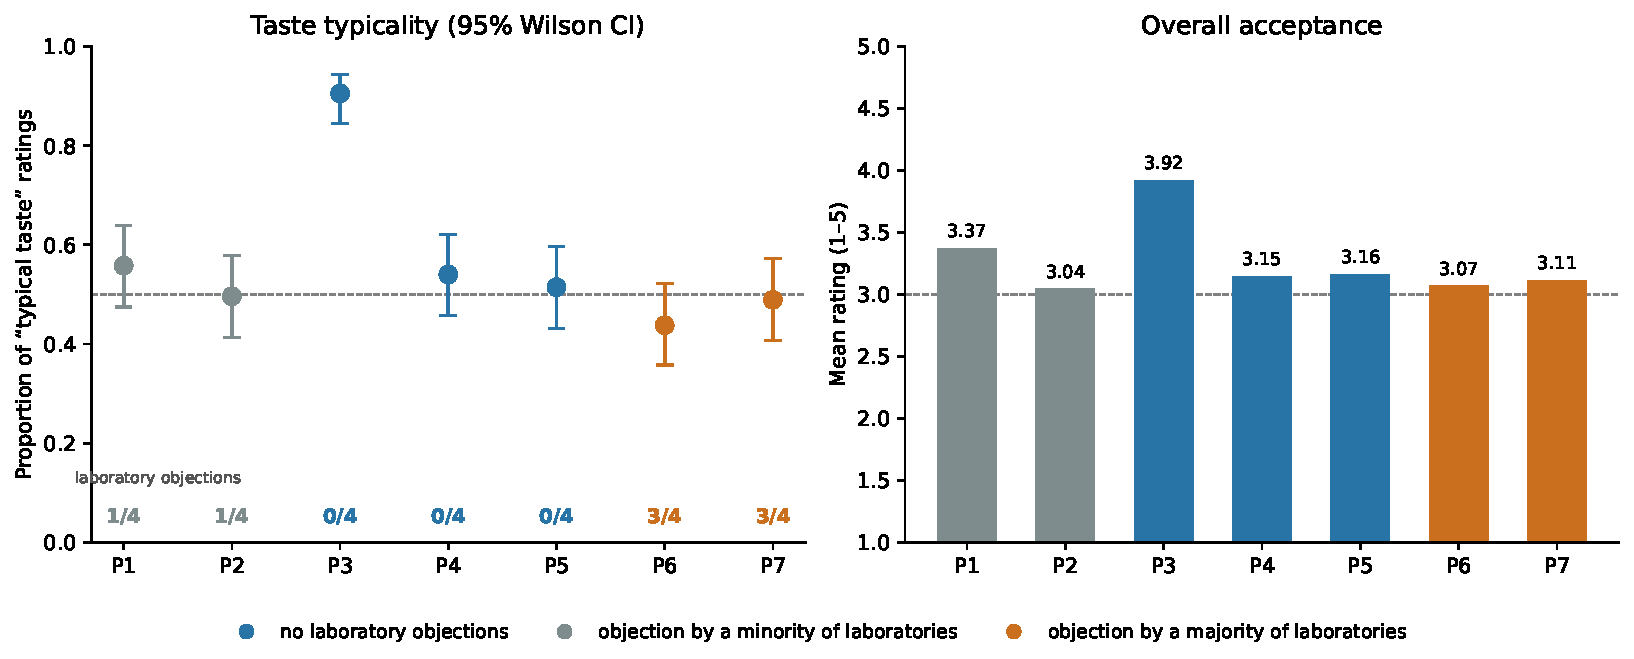
\includegraphics[width=16cm]{fig_panel_lab.pdf}
\end{adjustwidth}
\caption{Taste typicality (points, 95\% Wilson interval) and overall acceptance
(bars) of the seven samples in the blind consumer panel. Color indicates the
laboratory verdict: blue, no objections; grey, objection by a minority of
laboratories; orange, objection by a majority. Numbers at the bottom of the
left panel: number of laboratories (out of four) that rated the odor or taste
as not typical. Dashed lines: 0.5 and 3.\label{fig:panel_lab}}
\end{figure}

The samples flagged by the majority of laboratories (P6 and~P7) obtained
a typicality of 0.438 and 0.489 in the panel, lower than the mean
but indistinguishable from 0.5 ($p = 0.171$ and $p = 0.864$). In the
paired analysis, the typicality of the remaining samples
(P1, P2, P3, P4 and~P5: 0.603) was higher than that of the flagged samples
(0.464); the difference was $\Delta = 0.140$ (95\% CI:
0.071--0.208; $p < 0.001$; $d = 0.34$),
and for overall acceptance $\Delta = 0.24$ points
($p = 0.011$) (Figure~\ref{fig:contrast}). After excluding P3,
the difference in typicality fell to $\Delta = 0.064$ and was no
longer significant ($p = 0.109$).

\begin{figure}[H]
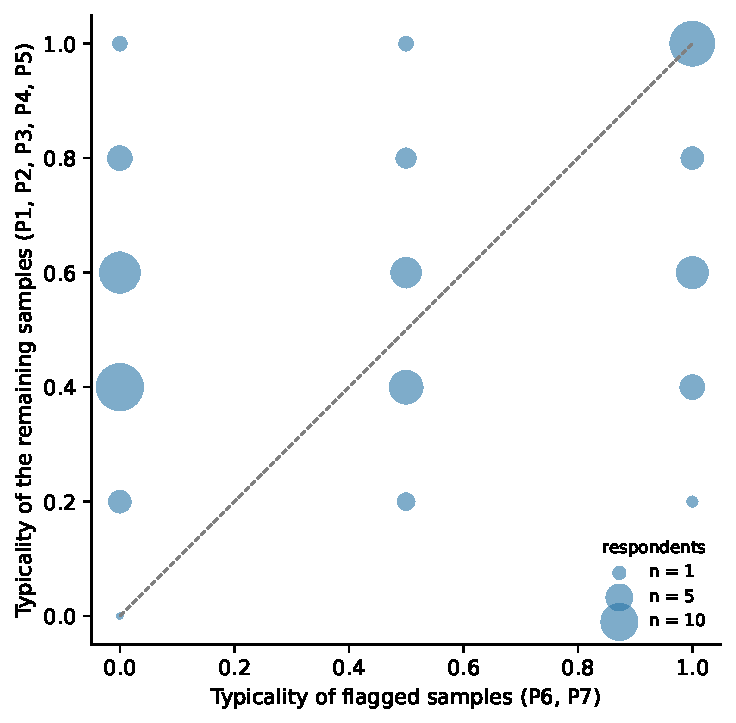
\includegraphics[width=8cm]{fig_contrast_lab.pdf}
\caption{Mean taste typicality of the samples to which the majority of
laboratories raised no objection ($y$-axis) and of the samples flagged by the
majority of laboratories ($x$-axis) for each respondent; point size: number of
respondents. Dashed line: equality of both ratings ($y = x$).\label{fig:contrast}}
\end{figure}

The panel did, however, register a feature consistent with some of the
laboratory descriptions: sweetness was rated as ``too strong'' most often for
P5 (41.3\%), P6 (40.9\%) and P7 (38.7\%), and least
often for P1 (22.1\%), P3 (22.6\%) and P2 (24.1\%).
Lab4 described the taste of P7 as ``very sweet'', which agrees with the panel
rating, but also the taste of P2, which the panel rarely rated as too sweet.


The blind consumer panel and the laboratories ranked the samples similarly in
terms of typicality, but they did not agree on which samples should be
considered not typical. The typicality ranking in the blind consumer panel
matches the laboratory ranking: sample~P3, to which the laboratories raised no
objections and which received the highest laboratory codes, was rated by far
the highest by consumers, whereas samples P6 and P7, flagged by three of the
four laboratories, were placed in the lower part of the ranking. Taste
assessment is therefore not devoid of content, since it reflects real
differences between honeys.

This agreement, however, rested on a single sample (P3), the only one
classified as typical by the blind consumer panel. After its exclusion, the
panel did not discriminate between the remaining six samples either in
typicality or in overall acceptance, and the typicality of P6 and P7 did not
differ significantly from 0.5: roughly half of the consumers considered the
taste of the samples flagged by most laboratories to be typical. The
difference between the flagged samples and the others was significant only
because of P3 and disappeared after its exclusion. The comparison on the same
scale shows this directly. The panel as a whole did not flag any sample, and
at the observed typicality a decision for P6 would require about
250~respondents. A single consumer agreed with a laboratory in 57.5\% of pairs
($\kappa = 0.10$), i.e., to a similar degree as with another consumer
($\kappa = 0.08$), whereas two laboratories agreed in 71.4\% of pairs
($\kappa = 0.30$). Typicality assessment thus recognizes clearly typical honey
but does not draw a sharp line between ``typical'' and ``not typical'' honey,
which is exactly the kind of line that a criterion of compliance with
commercial quality requirements needs.

\section{Discussion}

The consequences of low-quality organoleptic assessments have been described
most thoroughly for wine. In studies of wine judges, only about 10\% of them
were able to replicate their own rating of the same blind wine sample within
a single category \cite{hodgson2008judge}. Moreover, winning a high award at
one competition did not predict the result at another: the two results were
statistically independent \cite{hodgson2009concordance}. Organoleptic
assessment can be calibrated through the selection and training of assessors,
monitoring of panel performance indicators (repeatability, reproducibility,
agreement), and the use of reference standards and externally anchored scales
\cite{sipos2021panel,bartoshuk2004valid}. For honey, such a methodology was
developed within the International Honey Commission \cite{Piana2004}, and
since 1999 Italy has maintained a national register of experts in the
organoleptic analysis of honey, entry into which requires completed training
and a passed examination \cite{AlboMiele1999}. In France, the methodology for
the organoleptic assessment of unifloral honeys was developed by the team of
M.~Gonnet (INRA, now INRAE), whose work is the origin of modern organoleptic
analysis of honey \cite{Piana2004}. In Germany, the principles of the
organoleptic assessment of honey were drawn up by the German Agricultural
Society (DLG): its stated aims include the characterization of unifloral
honeys together with pollen analysis and the detection of the effects of
overheating and prolonged storage, and the assessment scheme lists, among
others, the odor and taste defects ``not typical for honey'', ``foreign
odor'' and ``fermenting'' \cite{DLG2015}. In both countries, organoleptic
assessment complements laboratory testing rather than replacing it. In routine
honey assessment, however, these indicators are usually not published in the
reports, and laboratories do not share a common reference material. The
comparability of organoleptic verdicts between laboratories thus remains an
assumption rather than a demonstrated property of the measurement.

The same pattern is evident between laboratories. Agreement among the four
laboratories was fair on the binary scale and slight on the three-level scale
\cite{LandisKoch1977}, and full agreement concerned only samples to which no
laboratory raised objections. Samples P1 and P2 were flagged by only one of
the four laboratories, while the others described them as typical, slightly
typical or of ambiguous characteristics. Lab4, which used a different method,
issued the verdict ``ambiguous characteristics'' for all seven samples,
including P6 and P7, which were flagged by the other three laboratories, and
reported an odor characteristic of signs of fermentation in three samples,
including P5, to which none of the other laboratories raised objections. The
verdict for the same batch therefore depends not only on random variability of
perception but also on the method applied and on the laboratory.

These discrepancies do not prove an error by any particular laboratory or a
defect of any particular batch. They do show, however, that in commercial
quality control practice the typicality of odor and taste is not measured
reproducibly between laboratories, in line with the predictions of the
psychometric literature
\cite{bartoshuk2003labeled,hodgson2009concordance,sipos2021panel}. The label
``not typical'' results from a comparison with an internal, implicit reference
of the assessor, and this reference differs between persons and laboratories.

\subsection{Describing an Attribute Versus Its Decision Weight}

The panel registered an attribute present in some of the laboratory
descriptions: the sweetness of P6 and P7 was rated as ``too strong'' more
often than that of other samples, and these samples received the lowest
typicality. This relationship was not unequivocal, however. Consumers
attributed the same sweetness intensity to sample~P5, to which the laboratories
using a typicality qualifier raised no objections. Sample~P2, in turn,
described by one of the laboratories as ``very sweet'', was rarely rated by
consumers as too sweet.

These results suggest that an organoleptic description may capture an
attribute of the sample accurately and still fail to distinguish typical from
not typical honey. A possible explanation is that typicality is determined not
by the intensity of a single attribute but by its consistency with the profile
of a given variety; this, however, requires further research. It is therefore
useful to distinguish an \emph{accurate description} from a \emph{decisive
criterion}: an attribute may be useful for characterizing a product and at the
same time unsuitable as a stand-alone basis for an administrative decision
\cite{Gajda2026}.

\subsection{Implications for Quality Control}

From the point of view of control, what matters is not whether taste
assessment carries any information at all, but whether it allows a verdict to
be reproduced. A single panelist rating reproduced the majority verdict of the
laboratories with $\mathrm{AUC} = 0.57$ (95\% CI: 0.54--0.60), and a rule
based on taste typicality would be wrong in nearly every second rating. The
agreement of a consumer with a laboratory ($\kappa = 0.10$) did not differ
from the agreement of two consumers ($\kappa = 0.08$). The laboratories
themselves fully agreed on three of the seven samples on the binary scale and
on one on the three-level scale. A criterion whose result for borderline
samples depends on the choice of assessor or laboratory does not satisfy the
condition of reproducibility and, when used on its own, the condition of
proportionality.

This difference is visible in the reports themselves. Lab2 and Lab4 described
a decision rule that takes measurement uncertainty into account
\cite[clause~7.8.6]{ISO17025} with respect to the limit values of measurable
parameters, and Lab4 explicitly named the physicochemical parameters and
pollen analysis. For the organoleptic assessment, no report stated an
uncertainty or a decision rule. For instrumental methods, precision is
determined in interlaboratory studies and is used to set critical differences
applied when assessing compliance with honey purity criteria
\cite{Ulberth2024}. For the verdict ``atypical taste'', no analogous
quantities are known.

This does not mean that organoleptic assessment is useless. It is a valuable
tool for studying preferences and for describing and improving products, and
also a signal for further testing, in the role foreseen for the organoleptic
test in the coordinated control plan of the European Commission
\cite{KE2015PlanKontroli}, when the result is extreme and consistent between
independent assessors, as for P6 and P7. A similar relationship has been
described for trained experts: in the International Honey Commission trials,
the results of assessing conformity with the profile of a unifloral honey were
valid for clearly good or clearly defective samples, whereas for samples with
intermediate characteristics the spread of ratings was largest, and the binary
``yes/no'' classification gave no valid result in 23\% of cases even after
three panels had been combined \cite{Piana2004}. The results indicate that for
borderline samples an organoleptic verdict should not be confirmed by a further
organoleptic assessment conducted without a reference. A second laboratory
using its own descriptors provides another description, not a decision: one
may describe the taste as ``very sweet'', another the odor as ``candy-like'',
and without a defined reference set of typicality descriptors neither
description establishes atypicality. The verdict ``atypical taste'' should
therefore be verified with reliable results, namely physicochemical and
microscopic determinations and, where adulteration is suspected, analytical
methods of known precision \cite{Ulberth2024}, before it becomes the basis for
a decision to withdraw a product. The role of organoleptic assessment in
commercial quality control should be limited to detecting the atypical
characteristics defined in the legislation, such as a foreign taste or odor
and signs of fermentation \cite{Dyrektywa2001110,RozporzadzenieMRiRW2009},
and should not extend to judging typicality, for which no reference exists.

Such a limitation corresponds to the structure of EU law. Directive
2001/110/EC formulates the organoleptic requirements as prohibitions: honey,
with the exception of baker's honey, must not have any foreign taste or odor
and must not show signs of fermentation \cite{Dyrektywa2001110}. An assessment
of appearance, odor, taste, consistency, crystallization and visible signs of
fermentation thus makes it possible to indicate a possible non-compliance and
to justify referring the sample for further laboratory testing. It was in this
preliminary and complementary role, and not as a stand-alone analytical
method, that the organoleptic test was used in the coordinated control plan of
the European Commission \cite{KE2015PlanKontroli}.

\subsection{Limitations of the Study}
\label{sub:limitations}

The main limitation is the small number of batches. Although the panel
provided 966~ratings, the sample-level comparisons (panel--laboratory
correlation, agreement of verdicts) are based on seven units. Second, the
panel consisted of consumers after a short briefing rather than of selected
assessors; this reflects the market perspective but increases the spread of
ratings. The panel question on taste typicality is also not identical to the
laboratory procedures, which assess odor and taste jointly according to their
own references. Third, the laboratory assessment was carried out as commercial
orders rather than as a formal proficiency test: the samples were not coded,
the laboratories had no common reference material, and the coding of their
descriptions on the T/L/N scale, including the assignment of code L to the
verdict ``ambiguous characteristics'', is a simplification made by the
authors. Fourth, the panel (May--July 2026) and the laboratory assessment
(August 2026) were separated by one to three months, during which
storage-dependent characteristics (crystallization, fermentation) may have
changed. Finally, only seven batches were examined, so the results should not
be generalized to all honeys.

\section{Conclusions}

The assessment of honey taste and odor typicality conducted as in this study
(by a blind consumer panel or by a single laboratory, without a common
reference standard and without a reported measure of assessor agreement) is
too variable to serve as a decisive parameter in the assessment of the
commercial quality of a sample.

Three independent findings support this conclusion. First, the discriminative
ability of the assessment is unacceptably low: a single panelist rating
reproduced the laboratory verdict with $\mathrm{AUC} = 0.57$, i.e., only
slightly better than a random binary choice ($\mathrm{AUC} = 0.5$) and clearly
below the value of 0.7 regarded as the minimum for acceptable discrimination
\cite{Hosmer2013}. In practice, the rule ``atypical taste, sample rejected''
would reject 39.7\% of the ratings of samples to which the majority of
laboratories raised no objections, and would pass 46.4\% of the ratings of
samples flagged by the majority, so it would be wrong in nearly every second
decision. Second, apart from one clearly typical sample, the panel did not
discriminate between samples and, as a whole, flagged none of them: the
typicality of the samples flagged by most laboratories (0.438 and 0.489) was
indistinguishable from 0.5. Third, the assessors agreed neither among
themselves nor with the laboratories: agreement among the four laboratories was
fair on the binary scale ($\kappa = 0.30$) and slight on the three-level scale
($\kappa = 0.13$), and a single consumer agreed with a laboratory to a similar
degree as with another consumer ($\kappa = 0.10$ and $\kappa = 0.08$).

A decision to accept a batch as compliant or to withdraw it, based solely on
such a result, would depend more on who assesses the sample and where than on
the properties of the sample itself. A subjective test should therefore not
serve as the basis for a binary ``good/bad'' judgment. Organoleptic assessment
retains its value as a descriptive tool and as a signal for further testing,
especially when the result is extreme and consistent between independent
assessors. It should not, however, decide on its own whether honey complies
with the commercial quality requirements. In the light of these results, the
distinction between identifying actual quality non-compliance and the
subjective evaluation of the organoleptic properties of honey is of central
importance. The absence of clearly defined and objective typicality criteria
limits the possibility of using the individual impressions of an assessor as
the basis for administrative decisions. In particular, terms such as ``too
sweet'', ``insufficiently aromatic'' or ``insufficiently typical'' do not in
themselves constitute evidence of a breach of quality requirements. Declaring
a product non-compliant on the basis of such assessments, without
demonstrating a link to a specific, legally defined criterion or to a
recognized or validated test method, may therefore raise serious doubts as to
the objectivity and legitimacy of the decision
\cite[Art.~34]{Rozporzadzenie2017625}.


\vspace{6pt}

%%%%%%%%%%%%%%%%%%%%%%%%%%%%%%%%%%%%%%%%%%
% Back matter. Every \tbc{...} must be completed by the authors before submission.
\authorcontributions{Conceptualization, B.L. and P.R.; methodology, B.L.; software, B.L.; formal analysis, B.L.; investigation, P.R. and J.R.; 
resources, P.R.; data curation, B.L.; writing---original draft preparation, B.L.; writing---review and editing, K.J.B., E.T., A.G., R.D., A.K.-D., J.R. and M.W.; visualization, B.L.; supervision, E.T, M.W..
 All authors have read and agreed to the published version of the manuscript.}

\funding{No external funding was received for the preparation of this manuscript. The article
processing charge (APC) will be covered by Stowarzyszenie Polska Izba Miodu (Polish Honey
Chamber Association). The APC funder had no role in the preparation of the manuscript or in the
decision to submit it for publication.}

\institutionalreview{ Not applicable.}

\informedconsent{Informed consent was obtained from all subjects involved in the study.}

\dataavailability{The anonymized panel data, the laboratory descriptions and the analysis code are available from the corresponding author upon reasonable request.}

\acknowledgments{During the preparation of this work, the authors used Claude Opus 5.5
(Anthropic) in order to improve the readability and language of the manuscript. The authors have
reviewed and edited the output and take full responsibility for the content of this publication.}

\conflictsofinterest{The authors declare no conflicts of interest}

%%%%%%%%%%%%%%%%%%%%%%%%%%%%%%%%%%%%%%%%%%
\abbreviations{Abbreviations}{%
The following abbreviations are used in this manuscript:\\

\noindent
\begin{tabular}{@{}ll}
AUC & area under the receiver operating characteristic curve\\
CI & confidence interval\\
DLG & German Agricultural Society (Deutsche Landwirtschafts-Gesellschaft)\\
IHC & International Honey Commission\\
L & slightly or weakly typical (laboratory code)\\
N & not typical for honey (laboratory code)\\
ROC & receiver operating characteristic\\
SD & standard deviation\\
T & typical (laboratory code)
\end{tabular}
}

%%%%%%%%%%%%%%%%%%%%%%%%%%%%%%%%%%%%%%%%%%
\appendixtitles{yes}
\appendixstart
\appendix
\section[\appendixname~\thesection]{Verbatim Odor and Taste Descriptions from the Laboratories}
\label{app:interlab_raw}

Table~\ref{tab:interlab_descriptions} lists the verbatim odor and taste
descriptions reported by the laboratories (August 2026,
Section~\ref{sub:interlab_methods}), which form the basis of the coding in
Table~\ref{tab:panel_lab}.

% Lab1--Lab3: English wording quoted from the original test reports (QSI reports are
% bilingual German/English; the English part is quoted). Lab4: translated from Polish
% (wording as in data/Analiza_porownawcza_ODER_23_2026.xlsx).
% Laboratory labels: Lab1 = QSI, Lab2 = Eurofins, Lab3 = Intertek, Lab4 = Puławy.
{\small
\begin{longtable}{@{}lc>{\raggedright\arraybackslash}p{5.2cm}>{\raggedright\arraybackslash}p{5.6cm}@{}}
\caption{Verbatim odor and taste descriptions reported by the four laboratories
for the same honey batches (August 2026). Lab1--Lab3: wording of the original
test reports (Lab1: English part of the bilingual German/English report); Lab4:
translated from Polish by the authors. The laboratory labels (Lab1--Lab4)
follow Table~\ref{tab:panel_lab}.\label{tab:interlab_descriptions}}\\
\toprule
\textbf{Sample} & \textbf{Lab.} & \textbf{Odor} & \textbf{Taste} \\
\midrule
\endfirsthead
\multicolumn{4}{c}{\tablename\ \thetable{} (\textit{cont.})}\\
\toprule
\textbf{Sample} & \textbf{Lab.} & \textbf{Odor} & \textbf{Taste} \\
\midrule
\endhead
\bottomrule
\endfoot
P1
 & Lab1 & not honey-specific & not honey-specific \\
 & Lab2 & animal urine-like, slightly source-specific & sweet, bloomy, mild, slightly source-specific \\
 & Lab3 & typical for honey & sweet, fruity \\
 & Lab4 & weak, slightly sour, characteristic of signs of fermentation & sweet, mild \\
\midrule
P2
 & Lab1 & not honey-specific & not honey-specific \\
 & Lab2 & animal urine-like, slightly source-specific & sweet, bloomy, mild, slightly metallic, slightly source-specific \\
 & Lab3 & slightly source-specific & sweet, fruity, slightly source-specific \\
 & Lab4 & unnatural, slightly floral & very sweet, prickling \\
\midrule
P3
 & Lab1 & source-specific & source-specific \\
 & Lab2 & slightly source-specific & sweet, bloomy, herbal, slightly source-specific \\
 & Lab3 & typical for honey & sweet, bloomy, fruity, herbal \\
 & Lab4 & strong, similar to beeswax & sweet, somewhat sharp \\
\midrule
P4
 & Lab1 & weakly source-specific & weakly source-specific \\
 & Lab2 & slightly honey-specific & sweet, fruity, medical, slightly metallic, slightly honey-specific \\
 & Lab3 & slightly source-specific & sweet, fruity, minty, slightly source-specific \\
 & Lab4 & faint, of rapeseed flowers & sweet \\
\midrule
P5
 & Lab1 & weakly source-specific & weakly source-specific \\
 & Lab2 & slightly source-specific & sweet, bloomy, medical, slightly bitter, minty, slightly source-specific \\
 & Lab3 & typical for honey & sweet, fruity, minty \\
 & Lab4 & distinct, characteristic of signs of fermentation & sweet, mild \\
\midrule
P6
 & Lab1 & not honey-specific & not honey-specific \\
 & Lab2 & absent & sweet, no specific floral aroma, not typical for honey \\
 & Lab3 & not typical for honey & sweet, fruity, malty, not typical for honey \\
 & Lab4 & strong, characteristic of signs of fermentation & sweet, reminiscent of burnt caramel \\
\midrule
P7
 & Lab1 & not honey-specific & not honey-specific \\
 & Lab2 & not typical for honey & sweet, no specific floral aroma, slightly metallic, not typical for honey \\
 & Lab3 & not typical for honey & sweet, fruity, malty, not typical for honey \\
 & Lab4 & strong, candy-like & very sweet, slightly prickling \\
\end{longtable}
}


%%%%%%%%%%%%%%%%%%%%%%%%%%%%%%%%%%%%%%%%%%
\begin{adjustwidth}{-\extralength}{0cm}

\reftitle{References}
\bibliography{bibliography}

\PublishersNote{}
\end{adjustwidth}
\end{document}
